  %%%%%%%%%%%%%%%%%%%%%%%%%%%%%%%%%%%%%%%%%%%%%%%%%%%%%%%%%%%%%%%%%%%%%%%%%%%%%
  %
%%%%%                    HEAD MATTER
 %%%
  %

\chapter{Evaluation}
%\addcontentsline{lof}{chapter}{\thechapter\quad Nihil Molestiae}
%\addcontentsline{lot}{chapter}{\thechapter\quad Nihil Molestiae}
\label{ch:evaluation}

\begin{quotation}
  {\small\it }"Everything that can be counted does not necessarily count; everything that counts cannot necessarily be counted"{\small\it -- Albert Einstein }
\end{quotation}



  %%%%%%%%%%%%%%%%%%%%%%%%%%%%%%%%%%%%%%%%%%%%%%%%%%%%%%%%%%%%%%%%%%%%%%%%%%%%%
  %
%%%%%                        FIRST SECTION
 %%%
  %
\section{Overview}
In this section we introduce the results obtained from the performance of the HBase-QoD framework. There are several ways of testing distributed systems, usually against each other, or compared to benchmark, or even to a centralized system. In this work, we compare mainly  the performance between the original version of HBase (or also called No-QoD in some parts of the graphs) and our proposal, HBase-QoD, by resorting to widely adopted benchmarks found in the literature.

Typically, performance in HBase improves as the number of servers increases due to more memory available~\cite{Carstoiu:2010}. In spite of that, scaling up HBase in cluster scenarios it is not always that trivial. Therefore, having alternatives for providing different levels of consistency to users, regarding data quality in cloud environments, may translate into substantial traffic savings. The associated cost saving to potential service providers or even customers, are a very relevant matter,  as seen in~\cite{chihoub:2013} for consistency-cost efficiency. Thus, it can be convenient to evaluate how selective replication (with a HBase-QoD in this case) can support that statement in distributed deployments with HBase.

\section{Experimental Testbed}
During evaluation of the HBase-QoD prototype a test-bed with several HBase cluster has been deployed at INESC-ID and IST in Lisbon, some of them with an HBase-QoD enabled engine for quality of data between replicas, and others running a regular implementation of HBase 0.94.8.

All tests were conducted using 6 machines with an Intel Core i7-2600K CPU at 3.40GHz, 11926MB of available RAM memory, and HDD 7200RPM SATA 6Gb/s 32MB cache, connected by 1 Gigabit LAN and we also simulate a Wide Area Network~\footnote{WAN, http://en.wikipedia.org/wiki/Wide\_area\_network} by using a network tool called netem~\cite{netem:2005} which can modify network latency between a distant set of locations.

We also explore how HBase-QoD affects bounds on data staleness, keeping it related to an upper limit (monitoring elapsed time, sequence of updates or just number of outstanding updates), by using the appropriate HBase-QoD configuration.

\section{Performance benchmarking suite}
In this section, we show the result of the experiments performed using with the Yahoo Cloud Service Benchmark~\cite{YCSB:2010}. This is a tool developed initially at Yahoo and later extended by some research fellows at Carnegie Mellon~\cite{Patil:2011} which aims at providing different metrics about distributed system scenarios. For instance:

\begin{enumerate}
\item RunTime in milliseconds.
\item Throughput in operations per second.
\item Number of Read, Update, Insert operations executed.
\item Minimum, Maximum and Average latency.
\item 95th and and 99th Percentile Latency.
\end{enumerate}

One of the most relevant performance metrics is throughput, and for us the aggregated average latency during insertions or transactions in the data store. Although, that does not fully show the real bandwidth usage we aim to represent. Therefore, and for the measurement of network bandwidth consumption and lag of replicated updates, an additional benchmark scripting module was developed by the author, as an additional assessment tool. Use of UNIX built-in tools such as \emph{tcpdump}~\footnote{http://www.tcpdump.org/} is extensively integrated into the script. Output data is represented with well-known tools such \emph{gnuplot}~\footnote{http://www.gnuplot.info/}.

\subsection{Workloads from YCSB}
First of all and for taking measurements, the CoreWorkload package of YCSB is used. A number of read/write workloads have been tested with the implementation of HBase-QoD and original HBase (no QoD bound). In addition, another custom workload with 100\% of writes (workload A-modified) is used in order to stress the database more intensively with writes. That is a more realistic and related testing scenario, as in the case of social networks (composed of mainly changes) , offering a continuous stream of updates so that simulations can be performed for the occasion. Later on, another two workloads with zipfian distribution are also tested using a more read focused percentage of operations (workload B). We perform these in order to realize what is the impact and differences between them and previous ones.

\begin{enumerate}
\item{YCSB workload A (R/W - 50/50)}
	\begin{itemize}
	Read/update ratio: 50/50
	\item Default data size: 1 KB records (10 fields, 100 bytes each, plus key)
	\item Request distribution: zipfian
	\item No HBase-QoD enforced.
	\item HBase-QoD fulfillment of $\sigma$=0.5\% of total updates to be replicated.
	\item HBase-QoD fulfillment of $\sigma$=2\% of total updates to be replicated.
	\end{itemize}

On the other hand, with HBase-QoD integrated into HBase, it is possible to have control over traffic of updates, which will go from being unbounded to up to a certain threshold, and subject to adjustments accordingly if there are needs for saving in resource utilization. We observe that a higher QoD (more updates are stored in Cache) exhibits less frequent network communication during the replication process, although peaks reach maximum values (on Bytes) as they need to send more data together. A lower QoD reduces peak-bandwidth usage but instead sends updates more frequently (this could be the case with wall posts in a social network).

\begin{figure*}
\centering
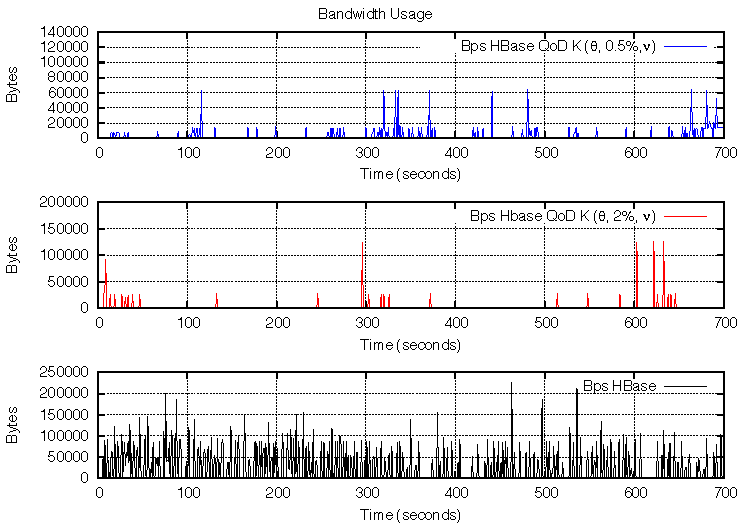
\includegraphics[scale=1.3]{figs/plot-packets-size-workloada-allbounds-latest.pdf}
\caption{Bandwidth usage for Workload A using 5M records using HBase-QoD bounds of 0.5 and 2\% for $\sigma$ of K.}
\label{fig-bandwidth-worloada}
\end{figure*}

Figure~\ref{fig-bandwidth-worloada} shows the results of three different sets of quality-of-data for \emph{workload A}. During the execution of the workload A, in Figure~\ref{fig-bandwidth-worloada}, the highest peaks in replication traffic are observed without any type of HBase-QoD, i.e. just using plain HBase. This is due to the nature of eventual consistency itself, and the internal buffering mechanisms in HBase. Naturally, without HBase-QoD updates are being replicated such as in best-effort~\footnote{Best-Effort delivery, http://en.wikipedia.org/wiki/Best-effort\_delivery} scenarios, where there is an unbounded limit on the number of updates shipped at a time and usually no data-semantics on which ones first or later. Therefore, the module here presented can adapt these limitations in cases of high traffic-loads, choosing first what matters more also.

%******************** TODO STOP ADD MORE text regarding this figure, one paragraph "readingT the graph" ***** DONE: A.G.R

\item{YCSB workload A modified (R/W - 0/100)}
	\begin{itemize}
	\item Read/update ratio: 0/100
	\item Default data size: 1 KB records (10 fields, 100 bytes each, plus key)
	\item Request distribution: uniform
	\item No HBase-QoD enforced.
	\item HBase-QoD fulfillment of $\sigma$=0.5\% of total updates to be replicated.	% 25K updates (5M total)
	\item HBase-QoD fulfillment of $\sigma$=2\% of total updates to be replicated.  % 100K updates (5M total)
	\end{itemize}


\begin{figure*}
\centering
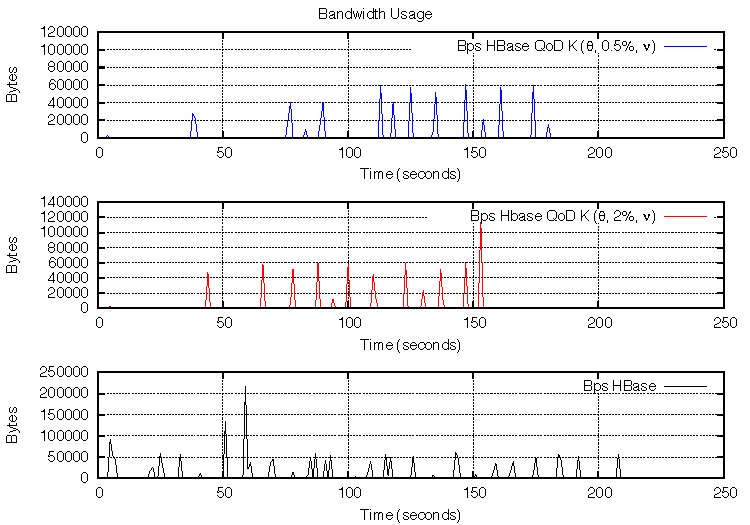
\includegraphics[scale=1.3]{figs/plot-packets-size-workloada-modified-allbounds-latest.pdf}
\caption{Bandwidth usage for Workload A-Modified using 5M records using HBase-QoD bounds of 0.5 and 2\% for $\sigma$ of K.}
\label{fig-bandwidth-worloada-modified}
\end{figure*}

In Figure ~\ref{fig-bandwidth-worloada-modified} we can see how a write intensive workload performs using a HBase-QoD deployment. Results obtained are outlined in the mentioned graph (please note the scale of the Y axis has been modified on each of the plots in order to make it convenient for showing the relevant difference in size more clearly).
  For smaller QoD (0.5\%), we see lower peaks in bandwidth usage, as well as in the following measurement used (2.0\%). Finally HBase with no modifications shows a much larger number of Bytes when it comes to maximum bandwidth consumption.

Note we are not measuring, or find relevant in any of these scenarios, to realize any kind of claims based on average bandwidth usage. The principal source of motivation of the work is to offer more flexible consistency semantics to users/developers, while also providing a way of controlling the usage of the resources in a data center; this resulting from  ensuring a uniform distribution of replication of updates across time. Also being able to trade strong consistency for grouping of operations that are treated atomically for shipment to a destination cluster location at a given point in time, or when the bounds on data-semantics are reached.\\


\item{YCSB - Workload B:}
\begin{itemize}
	\item Read/update ratio: 95/5.
	\item Default data size: 1 KB records (10 fields, 100 bytes each, plus key).
	\item Request distribution: zipfian.
	\item No HBase-QoD enforced.
	\item HBase-QoD fulfillment: $\sigma$=10\% of total updates to be replicated.
	\item HBase-QoD fulfillment: $\sigma$=20\% of total updates to be replicated.
\end{itemize}
	
\begin{figure*}
\centering
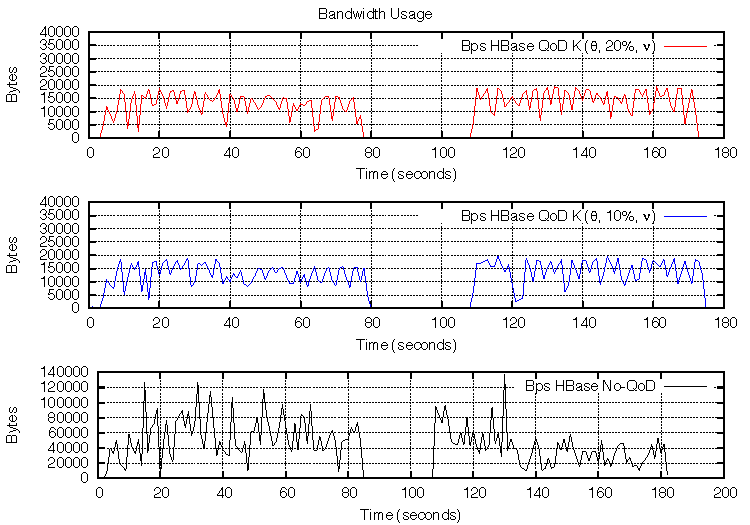
\includegraphics[scale=1.3]{figs/multiplot-size-workloadb-allbounds.pdf}
\caption{Bandwidth usage for Workload B using 500K operations in a total of 500K records using different HBase-QoD bounds for $\sigma$ in K.}
\label{fig-bandwidth-worloadb-10threads}
\end{figure*}

Figure ~\ref{fig-bandwidth-worloadb-10threads} shows the overall replication overhead with and without HBase-QoD, for a Read intensive workload. The graph is significantly different from previous workloads here presented in terms of updates being replicated. That is due to the small fraction of writes in the workload, when  compared to the percentage of items to which bounds on replication are being applied, using each of the QoD. If the QoD $\sigma$ value was too high, then the activity on the network would decrease for longer periods, replicating of updates rather later but in larger and higher bandwidth batches than with a lower QoD. Therefore, as a solution, increasing the amount of updates will result in more network traffic, but for this particular workload, it is still the case that a very limited amount of writes are going through the bounded HBase-QoD module.

\item{YCSB - Workload F:}
\begin{itemize}
	\item Read/update ratio: 50/50.
	\item Default data size: 1 KB records (10 fields, 100 bytes each, plus key).
	\item Request distribution: zipfian.
	\item No HBase-QoD enforced.
	\item HBase-QoD fulfillment: $\sigma$=20\% of total updates to be replicated.
	\item HBase-QoD fulfillment: $\sigma$=40\% of total updates to be replicated.
	\item HBase-QoD fulfillment: $\sigma$=60\% of total updates to be replicated.
\end{itemize}
\end{enumerate}

In the case of Figure~\ref{fig-bandwidth-worloadf-10threads}, lower QoD values for $\sigma$ slightly affect the height of the peaks of network communication during replication. This is due to the same reason as noted before: a bound on data staleness also puts a limit on the number of updates sent at the same time over the network. In the case of $\sigma$=60\%, the replication overhead is kept acceptable and constant in respect to the previous graph with $\sigma$=40\%. This is as well due to the number of updates issued during the workload, meaning that there is an upper limit reached in this type of scenarios, without the need, or advantage, to batch more updates per second, unless the number of operations is much larger for this particular workload. Later on, we see how the graph with QoD of $\sigma$=0\% (No-QoD in other words) has higher bandwidth consumption per second as expected.

\begin{figure*}
\centering
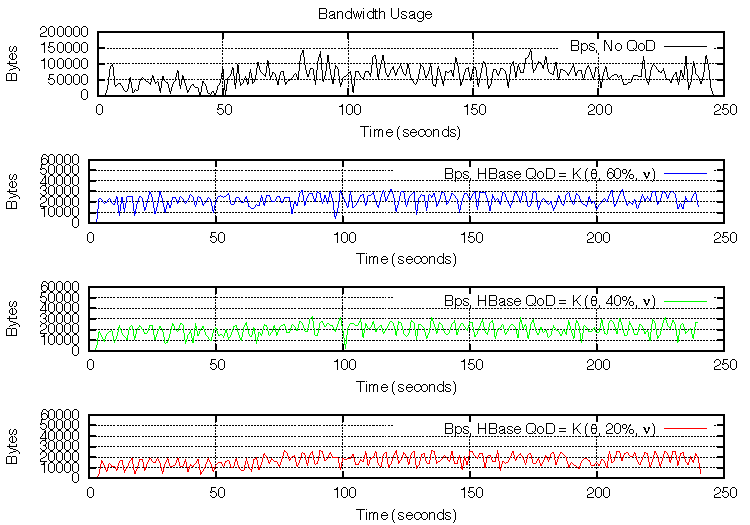
\includegraphics[scale=1.3]{figs/multiplot-size-workloadf-allbounds.pdf}
\caption{Bandwidth usage for Workload F using 500K operations in a total of 500K records using different HBase-QoD bounds for $\sigma$ in K.}
\label{fig-bandwidth-worloadf-10threads}
\end{figure*}

\section{Assessing data "freshness"}
\subsection{Data arrival measured on sets of updates received}
%\subsection{Extended workloads from YCSB++}

%%%% STOP TODO SEND THIS PARAGRAPH TO RELATED WORK IF SUITED
%YCSB++ is a project developed at Carnegie Mellon university and it has been recently published at an important conference venue, their authors claim to be able to extend the previous implementation of the benchmarking suite by Yahoo and therefore introducing the notion of measuring consistency and latency due to replication is a major tool improvement. In that case, also useful to experiments in the area of geo-replication as here described.

In order to assess data freshness, as observed by clients, a client is writing to a master cluster and another reading from the slave are set up. The writing client inserts 10 blocks of 100 updates interleaved between critical and non-critical into two different data containers with different QoD bounds. Therefore, it can be observed when and which type of update arrives at the destination by checking their delivery timestamp. That is also based on the data semantics offered by HBase-QoD.

\begin{figure*}[b]
\centering
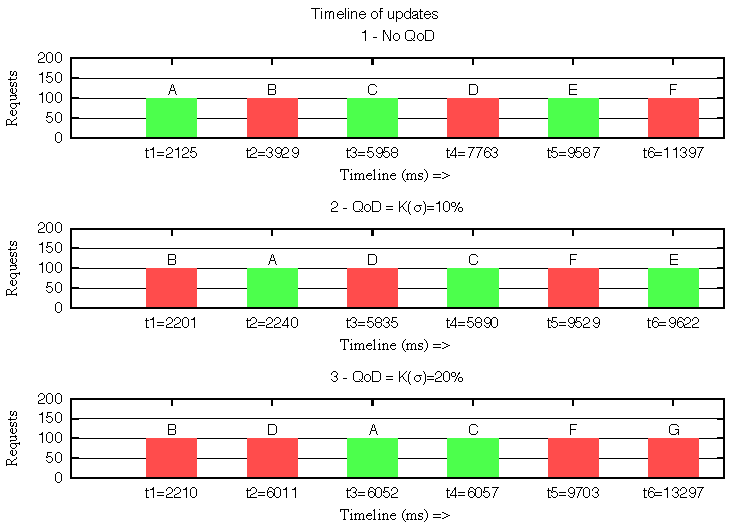
\includegraphics[scale=1.3]{figs/freshness-latest.pdf}
\caption{Freshness of updates with several HBase-QoD bounds}
\label{fig-freshness-letters}
Critical updates (in red)
Non-Critical (in green)
\end{figure*}

In Figure~\ref{fig-freshness-letters}, we show how the latency varies by referring to the update timestamps. Higher QoDs approximate critical updates (in red) more to the beginning of the \emph{Timeline}, while non-critical (green) keep being moved towards the right (later reading). We have therefore a better data freshness metric, in terms of critical updates, by prioritizing them through our HBase-QoD. Critical updates move closer to the left side of the X axis with an increasing $\sigma$ bound in K vector, so that is actually giving them higher priority during the replication process.

\subsection{Data arrival measured in a per update basis}
In this setup there is a client writing to a master HBase server using HBase-QoD ,which writes 1000 updates randomly mixed between critical and non-critical. We are introducing a delay of 40ms in the network in order to realize that wide are network assumption: the delay is set between master and slave cluster communication. For best readability, we are just showing a subset of the updates sent over time, from client 1 to the master cluster, and later read by client 2 from the replica at the slave cluster.

In Figure~\ref{fig-baseline-critical-vs-non-critical} it is represented the result of a set of updates applied onto two different data containers. Each of them having at least two QoD bounds applied to shipping and replication logic. That is, namely the K($\sigma$) in the vector we previously describe. We represent the arrival times for all types of updates, critical and non-critical, in each of the QoDs.

\begin{figure*}[h]
\centering
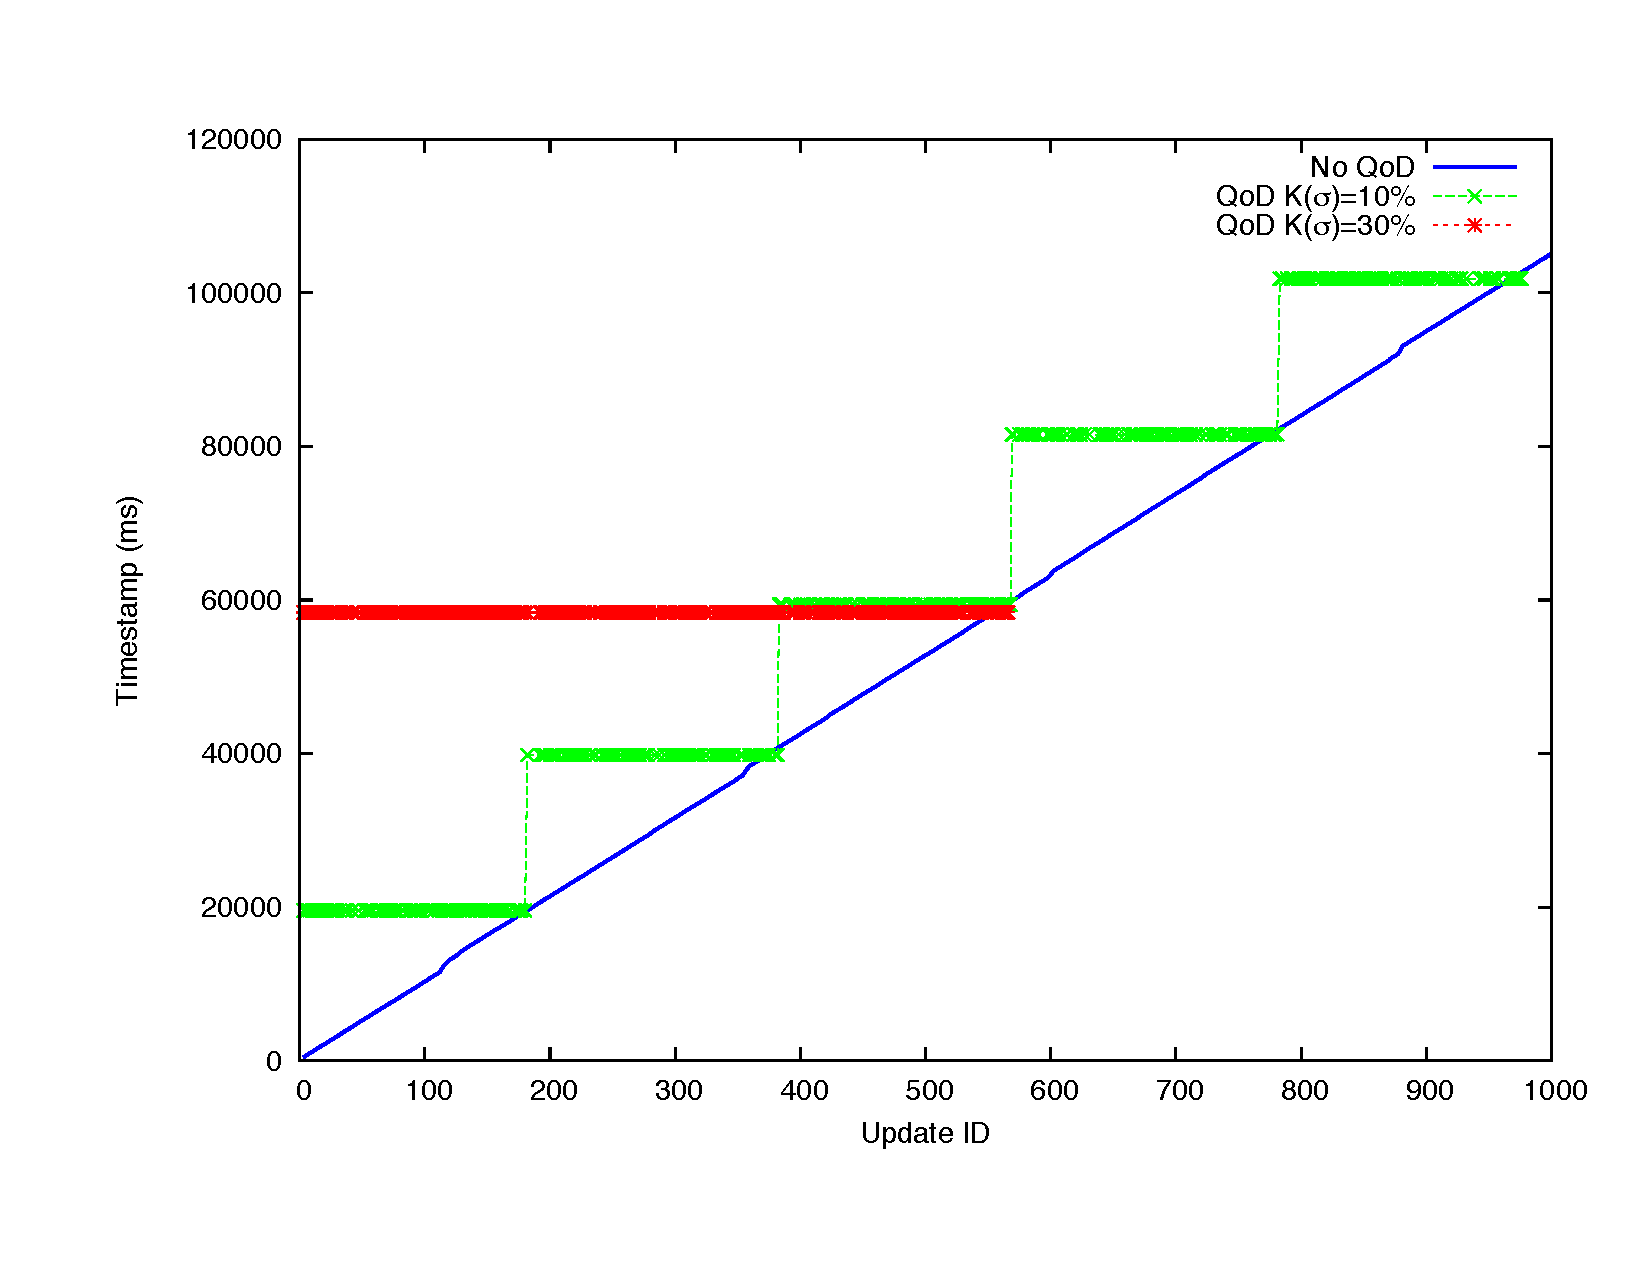
\includegraphics[width=1.0\textwidth]{figs/timestamps-non-critical-updates-false.pdf}
\caption{Difference in arrival times with and without QoD for non-critical updates}
\label{fig-baseline-critical-vs-non-critical}
\end{figure*}

Regarding maximum delay given the type of update, non-critical updates will have higher timestamp than the others and therefore arrive later, while in the case of critical, as shown in graph~\ref{fig-baseline-critical-vs-non-critical} they get read earlier in comparison to the base No-QoD line in many occasions. It is important to note these are types of updates for each QoD (green and red) so one needs to take into account that not all updates exhibit the same behavior, but approximately non-critical always arrive later on or equal to baseline No-QoD while critical ones do the opposite. This is expected in the graph and the goal is simply to realize how the Cache mechanisms perform the caching plus flushing of updates over time.

\begin{figure*}[h]
\centering
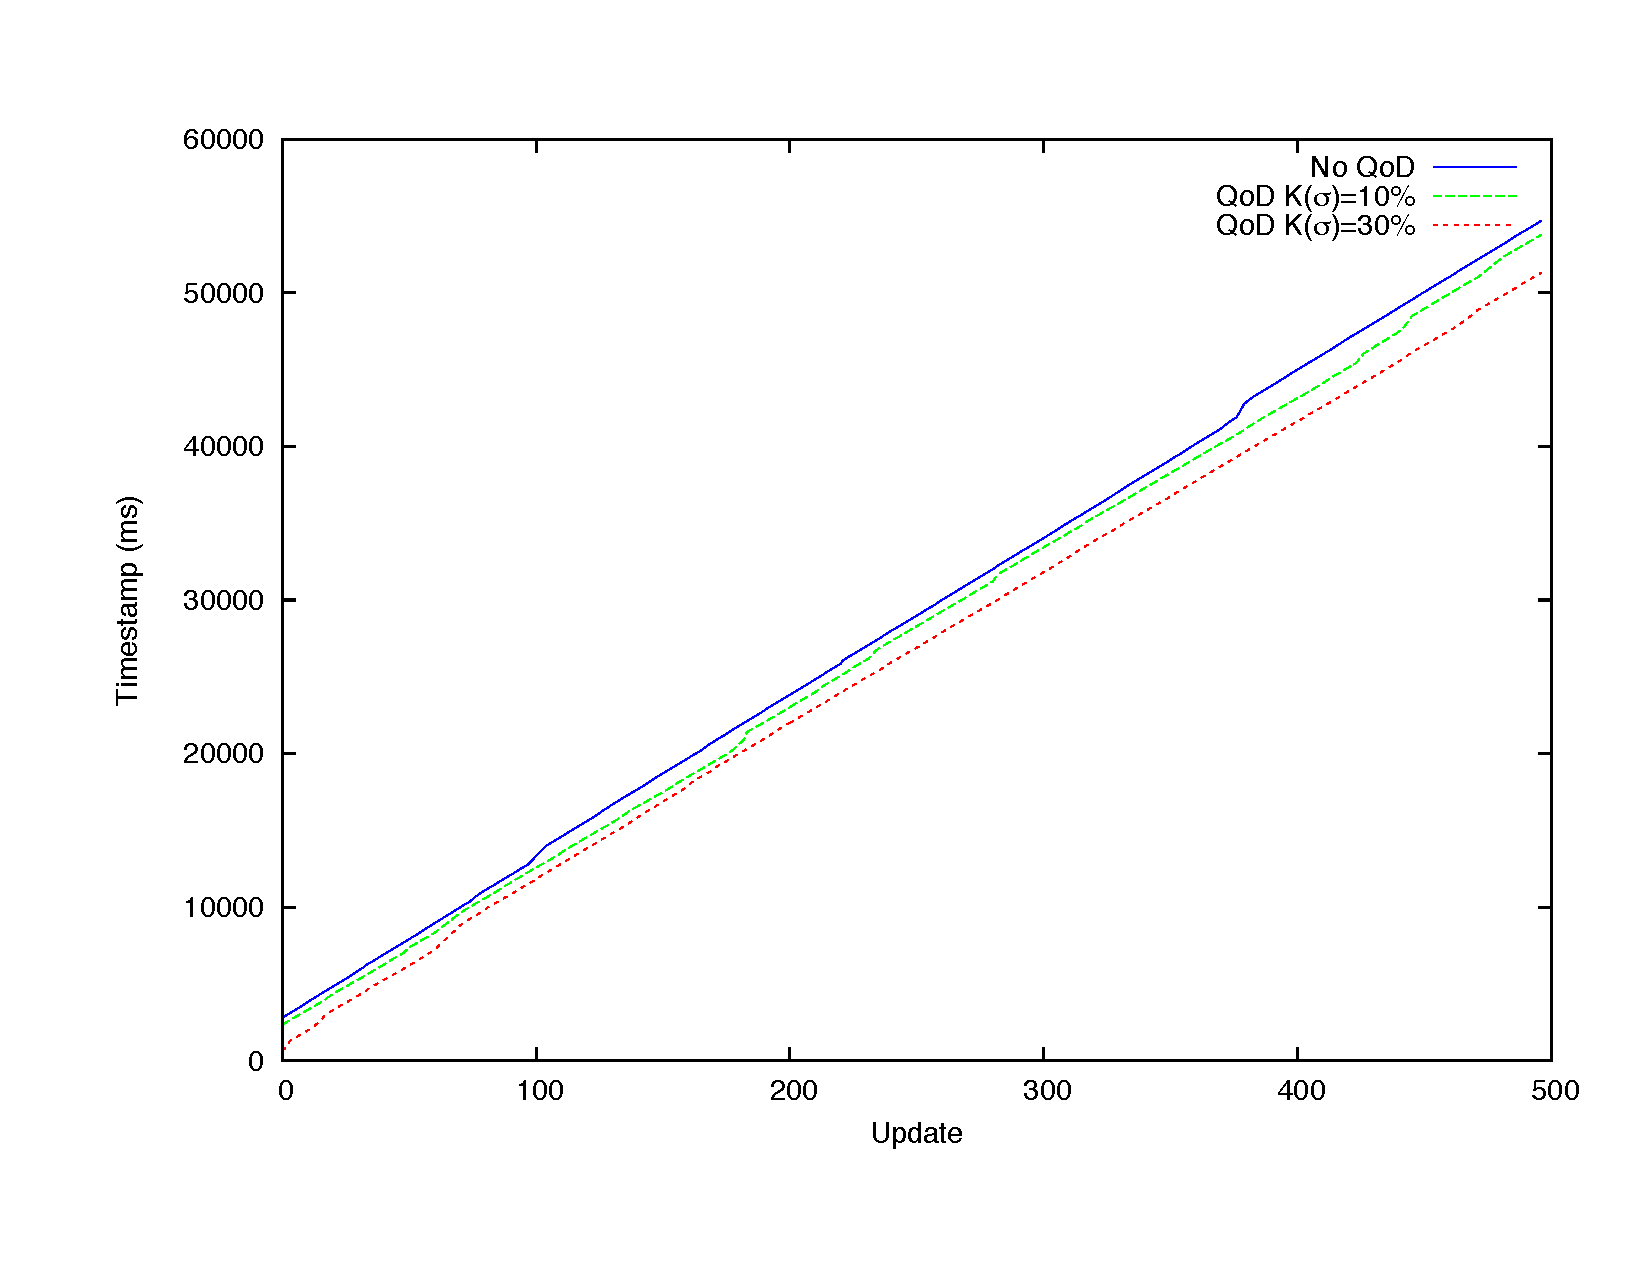
\includegraphics[width=1.0\textwidth]{figs/timestamps-critical-updates.pdf}
\caption{Difference in arrival time with and without QoD bounds for critical updates}
\label{fig-timestamps-critical-updates}
\end{figure*}

In Figure~\ref{fig-timestamps-critical-updates}, the graph highlights how more critical updates arrive earlier in a per update basis over time. The more stringent is the QoD bound, the earlier critical updates are received, made available to, and read by another client from the slave cluster. The more latency or network overhead are there, the higher this difference appears to be.

\section{Overall Performance and Resource Utilization}
In Figure~\ref{fig-bw-freq}, for a very small QoD of K using $\sigma$, we observe that there is a lowest limit where latency can not be reduced any further. We have realized that same limit exists in the previous Figure~\ref{fig-bandwidth-worloada-modified} when using a larger QoD of K using $\sigma$ = 0.5\%. Please note updates that need to be applied prior to replication (QoD percentage), are so in relation to the total number of operations in the workload (a very small value means a more stringent QoD, the lowest possible value for that is of approximately of 0.00\% and that would be just the strictest bound possible on QoD).

We can see the bandwidth peaks, and therefore measure average usage of the bandwidth, which decreases with the increase of the QoD bound; in the order of magnitude of 1MB per second, as we experimentally verify from the graphs obtained. That is due to the batching of updates in our consistency model, so items are not replicated until one of the constraints time, sequence or value is met. Basically, overall we can see less communication between clusters at replication time with increasing QoD, which is a good measurement of how one can optimize bandwidth. During that time then, we take advantage of our caching mechanisms inside HBase-QoD while sending all the information demanded in a timely fashion once recent data becomes being considered necessary to the application (depending on the QoD).

We also confirm that HBase-QoD does not hurt performance, as we observe from the throughput achieved for the several levels of HBase-QoD chosen during the evaluation of the throughput with the benchmark for our modified version with HBase-QoD enabled, in Figure~\ref{fig-throughput}. The differences in throughput are irrelevant and mostly due to noise in the network, that is the conclusion after obtaining similar results to that one in several rounds of tests, with the same input workload on the data store.

Additionally, we also conducted an experiment to monitor the comparative CPU usage load, in a HBase system using HBase-QoD. This is shown in Figure~\ref{fig-cpu}, and \emph{dstat} presents. CPU consumption and performance remains roughly equivalent, and therefore stable in the cluster machines.

Finally there is an "overhead", if it can be called like that, regarding the wide-spread of replication activity over time if information is kept into memory (caching mechanism of HBase-QoD) for too long before actually replicating occurs. But that is expected and acceptable, namely taking into consideration the results obtained and traded for reduced maximum peak-values in network bandwidth.

\begin{figure}[b]
\centering
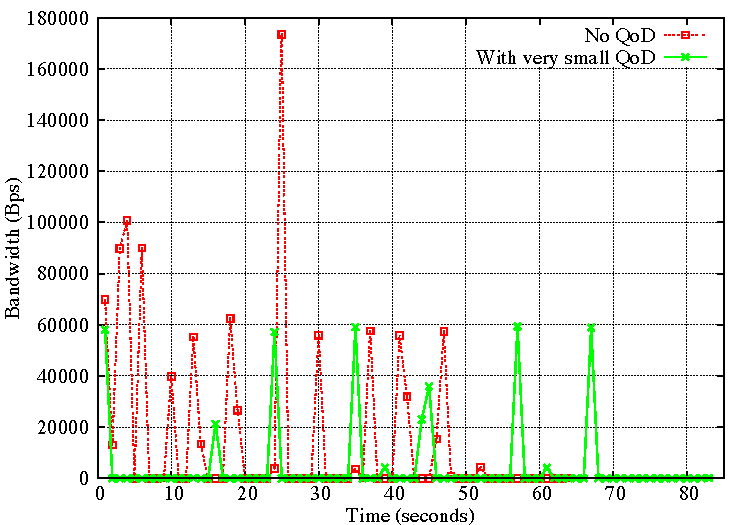
\includegraphics[width=0.8\textwidth]{figs/bandwidth.pdf}
\caption{Bandwidth usage and replication frequency for a typical workload with and very small HBase-QoD constraint for K($\sigma$)}
\label{fig-bw-freq}
\end{figure}

\begin{figure}[b]
\centering
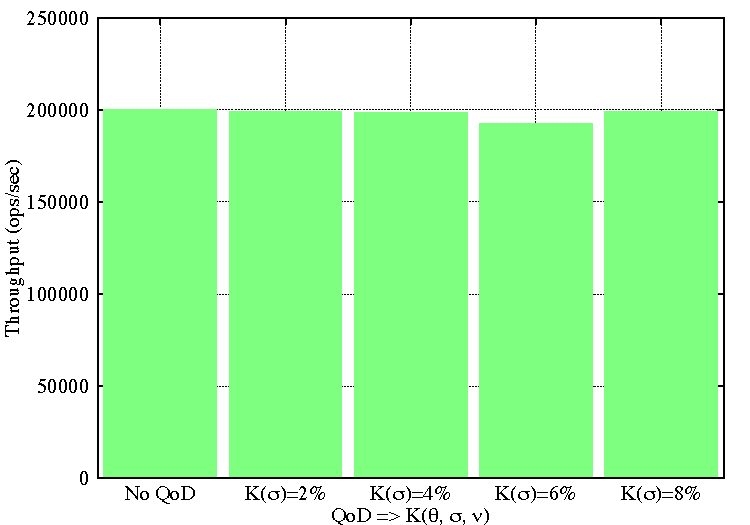
\includegraphics[width=0.8\linewidth]{figs/throughput.pdf}
\caption{Throughput for several HBase-QoD configurations}
\label{fig-throughput}
\end{figure}

\begin{figure}[b]
\centering
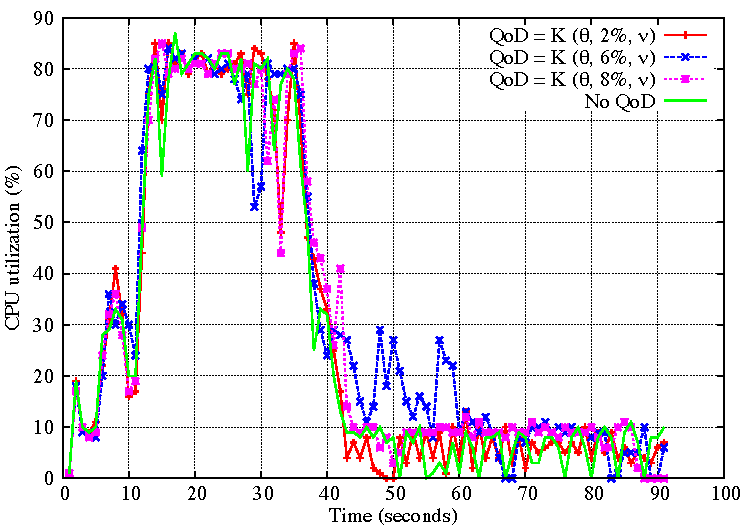
\includegraphics[width=0.8\linewidth]{figs/cpu.pdf}
\caption{CPU usage over time with HBase-QoD enabled}
\label{fig-cpu}
\end{figure}

%In Figure 1, we appreciate that our HBase-QoD helps to control peak bounds of updates, and therefore the eventual consistency approach of leaving replication of the items at the odds of the RPC mechanisms of the system in question. We %can control that, and the graph shows how a maximum threshold of around 1000 is constantly reached for the modified version of HBase, but no more. Obviously the timespan of updates with HBase-QoD might be longer depending of the values %chosen, but that is a built-in property of our work on purpose for only propagating updates when they are strictly necessary and to satisfy a given SLO.

%In Figure 4 (for batches of updates of 5M) we can see the bandwidth peaks and therefore measure average usage of the former, which decreases with the increase of the HBase-QoD bound in the order of magnitude of 1MB per second as we experimentally verify from the graphs obtained. That is due to the batching of updates in our vector model, so items are not replicated until one of the constraints time, sequence or value is met. Overall we see less communication between clusters at replication time if there is an increasing value of sigma in the HBase-QoD, which is a good measurement of how one can optimize for bandwidth while non-key data semantics are presented to the application at just the required instant in time but not earlier unless a critical update. During the time where replication is not triggered we take advantage of the caching mechanisms inside HBase-QoD, later sending data as it necessary to the application.

\subsection*{Summary}
In this chapter, we described the evaluation of the presented HBase-QoD framework, regarding its performance, semantics, and resource utilization. This was carried out by comparative assessment between the original version of HBase (No-QoD) and HBase-QoD, making use of widely adopted benchmarks found in the literature.
The HBase-QoD prototype was evaluated with a test-bed of HBase clusters at INESC-ID and IST in Lisbon, some of them with an HBase-QoD enabled engine for quality of data between replicas, and others running a regular implementation of HBase 0.94.8.
Globally, the results reinforce the purpose of HBase-QoD and are in line with what was expected, across a variety of YCSB-derived workloads, regarding overall bandwidth utilization and its peak usage, update latency (and application semantics), as well as CPU utilization.
